\documentclass{article}
% \documentclass[10pt]{article}
\usepackage[margin=1.7in]{geometry}
\usepackage{etoolbox}
\pagenumbering{arabic}
\input{preamble}
\newcommand{\stzh}[1]{{\color{blue}[stzh: #1]}}

% 🥚 ULTIMATE EASTER EGG 🥚
% If you're reading this, you've found the secret message!
% 
% Dear future cryptographers and privacy advocates,
% 
% You've stumbled upon a whitepaper that represents a significant step forward
% in the quest for true digital privacy. Anysphere isn't just another messaging
% app - it's a glimpse into a future where your conversations are truly private,
% where metadata doesn't betray your secrets, and where "no needless trust"
% isn't just a slogan but a fundamental principle.
%
% The easter eggs scattered throughout this codebase are our way of saying:
% even the most serious cryptographic work deserves a smile. After all,
% if we can't have fun while building the future of privacy, what's the point?
%
% Remember: Alice and Bob have been trying to talk privately since 1976.
% Let's finally give them (and everyone else) the tools they deserve.
%
% Stay paranoid (in the best way),
% The Anysphere Team
%
% P.S. - If you found all the easter eggs, you deserve a coffee. ☕
% P.P.S. - Yes, we know there are probably bugs. It's crypto software. 🐛
% P.P.P.S. - The rubber duck debugging method works surprisingly well for PIR queries. 🦆

\title{\vspace{-2cm} \textbf{\Large Anysphere: Private Communication in Practice} \\ \vspace{0.3cm} {\large \normalfont Security Whitepaper} \vspace{-0.1cm}}
\def\dateinfo{July 6, 2022\\ \vspace{0.2cm} \textit{Last updated:} \today}
\date{\normalsize \dateinfo}
\author{\normalsize Arvid Lunnemark \hspace{0.7cm} Shengtong Zhang \hspace{0.7cm} Sualeh Asif \vspace{0.1cm} \\ \normalsize \nolinkurl{{arvid, stzh1555, sualeh}@anysphere.co}}

%\setshortauthors{Arvid Lunnemark, Shengtong Zhang, Sualeh Asif}
%\setshorttitle{Anysphere: Private Communication in Practice}

\makeatletter
\patchcmd{\@maketitle}{\begin{center}}{\begin{adjustwidth}{-0.5in}{-0.5in}\begin{center}}{}{}
\patchcmd{\@maketitle}{\end{center}}{\end{center}\end{adjustwidth}}{}{}
\makeatother

\begin{document}

\maketitle


\begin{abstract}
	\noindent We describe Anysphere, a metadata-private communication system deployed in the real world. Using private information retrieval(PIR) based on homomorphic encryption, our protocol guarantees security \xxx[stzh]{metadata-privacy?} even if all of our servers are compromised and any number of the users and network observers are malicious. In this whitepaper, we precisely define our threat model, and show how we achieve security against it both in theory and in practice.
\end{abstract}



%\tableofcontents

\section{Introduction}

When the internet was first established, everything sent over it was public. If A sent a message to B, anyone on their path through the internet could see that such a message was sent, and read the actual message. As of today, many messaging services are end-to-end encrypted, meaning that no one can read the contents of messages. However, for sufficiently powerful adversaries, it is still possible to find out who is talking to whom. The goal of private communication is to hide this metadata: we want to create a system where A and B can send messages to each other over an untrusted network, without anyone knowing that they talk to each other. Such a private communication system would be critically important to protect and expand freedom in the world \cite{arvid}.

Anysphere is a provably secure metadata-hiding communication platform, built for the real world. In this document, we outline how we guarantee theoretical security, and how we make sure that the theoretical security translates to good practical security.

\section{Security Context}
\label{sec:securitycontext}

\todo{Explain why Signal is not enough. Good table.}

In this section, we describe what our system achieves beyond end-to-end encrypted messaging applications like Signal and Wickr.

Signal is great. It is end-to-end encrypted, open source, and run by a trustworthy group. Unfortunately, if their servers are hacked, one of their employees bribed, or you are simply attacked by a network-level powerful actor, there is nothing Signal can guarantee. \xxx[stzh]{This is not true. The point of E2E encryption is to guarantee content security when the server gets compromised.}

Furthermore, even with a secure server, it leaks metadata. Using timing attacks, an adversary can figure out when, where and with whom you are talking. 
\subsection{Goals}

Our goal is to provide metadata protection in the presence of a powerful adversary. More precisely, we want to achieve

1) Metadata privacy for communication: if Alice and Bob use Anysphere to communicate, then an adversary who controls everything other than Alice and Bob's Anysphere client shouldn't be able to tell whether Alice and Bob are engaging in a conversation at any point in time.

2) Metadata privacy for trust establishment: if Alice and
\section{Threat Model}

\todo{add table comparing our threat model with e.g. signal and email}
\todo{add an illustration of a walled garden, with the walls containing only your computer and your friends' computers}

%Touch on: server, friends, client-side computer, etc.

\todo{Figure out a better format here. See e.g. Skiff's whitepaper.}



Similar to most PIR schemes(for example \cite{ahmad2021addra}, \textsection 2.2), our threat model assumes a global adversary who can compromise the entire communication infrastructure except for the user's and their friends' client end. In particular, we assume the adversary has control over all the servers, and can observe and manipulate all network traffic.

End-user trust is more subtle matter. In \cite{angel2018s}, Angle, Lazar and Tzialla describes the compromised friend(CF) attack on a general meta-data private messaging system, which shows that perfectly hiding metadata while not trusting the user's friends is computationally prohibitive. In our security model, a user trusts that the devices of themselves and all their friends are uncompromised and running an unmodified copy of anysphere's client-side code. The user assumes that any other end-user device might be compromised.

\todo{Can we assume that only a small number of friends are compromised?}

Finally, we assume the security of the standard cryptography primitives we use, including microsoft SEAL's BFV cryptosystem and libsodium's AEAD cryptosystem. 

Denial of Service(DoS) attacks are unavoidable if the adversary controls all our servers. In the case of such attacks, we do not guarantee liveliness of our service, but continue to guarantee metadata security. We also defend against DoS attacks launched by an end-user with no access to the servers.

\subsection{Desired Properties}

1. \textbf{Perfect Metadata Protection}: All contents and metadatas associated with a conversation are only visible to the users involved with the conversation. Even with a compromised server, an adversary should not even be able to find out whether two users are engaging in any conversation.

2. \textbf{Forward Secrecy}: \todo{do we provide this?}

3. \textbf{Resistant to man-in-the-middle attacks}.

4. \textbf{Resistant to social engineering attacks}.

\todo{add more.}




\section{Core Protocol}
\label{sec:coreprotocol}

Consider two fictional users, Alice and Bob. Alice and Bob want to message each other over an untrusted network without leaking any data or metadata to anyone. They use authenticated end-to-end encryption to hide the message content and ensure integrity. They employ two key ideas to hide metadata: sending data at a constant rate and retrieving homomorphically compressed data.

When signing up, each user gets their own \textit{outbox} on the server, which is a dedicated storage space for their messages. Once every minute, Alice sends exactly $1$ KB of data to her outbox. If she has a message to send, she sends the padded encryption of that message. Otherwise, she sends a random sequence of bytes. This simple idea ensures that neither the server nor network observers know when Alice sends a real message.

Our next problem is how to route the message to Bob. In a traditional messaging system, Bob downloads data from Alice's outbox and decrypts it. However, this leaks metadata: the server learns that Bob read from the Alice's outbox.

One solution is for Bob to, once every minute, download \textit{all} outboxes from the server. He can then check the value of Alice's outbox locally. This way, it is impossible for the server to link Alice to Bob.

This simplified scheme is almost how Anysphere works. Unfortunately, Bob cannot download all outboxes every minute — that would be too much data! Instead, he uses \textit{private information retrieval}, a well-studied cryptographic primitive, to compress his download size. \Cref{fig:highlevelpir} illustrates the core protocol. The following subsections will describe the system in detail.

% make this take up both columns at the top of the page
\begin{figure}
    \centering
    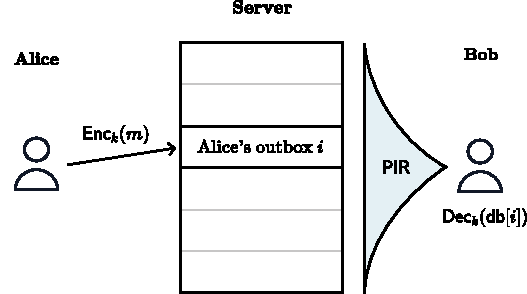
\includegraphics[width=0.7\textwidth]{pirfigure.pdf}
\caption{Alice sends the encryption of a message $m$ to her outbox once every minute. Bob retrieves Alice's outbox using private information retrieval (PIR), which appears to everyone else but Bob as if he had downloaded any outbox. Alice and Bob can use standard symmetric encryption to communicate, and the server will not learn anything at all.}
\label{fig:highlevelpir}
\end{figure}

\subsection{Private information retrieval}

We view the outboxes as an array, called $\db$. Bob wants to download Alice's outbox $\db[i]$ without revealing $i$ to anyone. This problem was first introduced as \textit{private information retrieval} (PIR) in 1995 \cite{chor1995private}, extended in 1997 to our threat model under the name cPIR \cite{kushilevitz1997replication}, and has been extensively studied since then \cite{melchor2016xpir,angel2018pir, ahmad2021addra}.

All known cPIR schemes use homomorphic encryption \cite{gentry2010computing}. To compute the query $q$, Bob encrypts $i$ with a homomorphic encryption scheme using a secret key $s$. That is, $q = \mathsf{HEnc}_s(i)$. The server can then homomorphically evaluate the function $f(i) = \db[i]$, producing the answer $a = \mathsf{HEnc}_s(\db[i])$. Bob can finally decrypt to find $\db[i]$. In practice, $f(i)$ is often defined in terms of a dot product with a unit vector representing $i$, because BFV, the homomorphic scheme being used, \cite{fan2012somewhat}, is particularly good at dot products.

Our implementation currently uses FastPIR, one of the fastest cPIR schemes \cite{ahmad2021addra}. All cPIR schemes have the same security properties, and we are actively researching faster schemes (see \cref{sec:future}).

\subsection{Security}

The simplest version of our core protocol is shown in \cref{fig:simple}. In this section, we show (1) that Alice and Bob enjoy metadata privacy without having to trust anyone else, (2) that our system guarantees message integrity, and (3) that our protocol is resistant to denial of service attacks from users.

We define security in the simulation sense \cite{lindell2017simulate}. To do so, we first need to define what an attacker learns, which includes both the data sent from all users to the server along with timestamps, as well as the local keys on attacker-controlled devices. Let $(S, i, \mathsf{tk}, c, t)$ represent the data sent to the server in the sending phase at time $t$, let $(R, q, t)$ represent the data sent to the server in the retrieving phase at time $t$, and let $(A, a, t)$ represent the data sent from the server in response to the retrieval request at time $t$. Our protocol does not operate in rounds, so $t$ can be any real number.

We say that a private communication scheme consists of the four algorithms $(\pcalgostyle{Register}, \mathsf{Send}, \mathsf{Receive}, \mathsf{Route})$, where $\pcalgostyle{Register}$ registers the user and generates a secret key

\begin{definition}[Metadata privacy]
    We say that a private communication scheme $(\pcalgostyle{Register}, \mathsf{Send}, \mathsf{Receive}, \mathsf{Route})$ is \textit{metadata-private} if for all $n = n_\lambda = \poly(\lambda)$, all $\mathcal{K} = \mathcal{K}_\lambda \subseteq [n]$, all $T = T_\lambda = \poly(\lambda)$, all user functions $m_u$, $t_u$ and $j_u$, all efficient attackers $\mathcal{S}$, and all efficient distinguishers $\mathcal{A}$, there exists an efficient algorithm $\mathsf{Sim}$, such that the following two probability ensembles, parametrized by $\lambda \in \N$, are computationally indistinguishable:
    \begin{align*}
        \Dreal &= \left\{ 
        \begin{aligned}
          (\{h_u^T\}_{u \in [n]}, &\{ \sk_u \}_{u \in \calK}, \{ t_u \}_{u \in [n]}) \colon \\
          \sk_u &\gets \pcalgostyle{Register}(1^\lambda, u) \;\; \forall u \in [n]\\
          h_u^0 &\gets \emptyset \;\; \forall u \in [n] \\
          s_u^{i+1} &\gets \mathsf{Send}(m_u(h_u^i), t_u(i), \sk_u) \;\; \forall u \notin \mathcal{K} \\
          q_u^{i+1} &\gets \mathsf{Retrieve}(j_u(h_u^i), t_u(i), \sk_u) \;\; \forall u \notin \mathcal{K} \\
          h_u^{i+1} &\gets h_u^i \cup s_u^{i+1} \cup q_u^{i+1}  \cup \mathcal{S}\left(H_t, q_u^{i+1}\right) \;\; \forall u \notin \mathcal{K} \\
          h_u^{i+1} &\gets h_u^i \cup \mathcal{S}(H_t) \;\; \forall u \in \mathcal{K}
        \end{aligned}\right\}_{\lambda \in \N}\\
        \Dideal &= \left\{
        \begin{aligned}
          \Sim\big(1^\lambda, \{h_u^T\}_{u \in \calK}, &\{ \sk_u \}_{u \in \calK}, \{ t_u \}_{u \in [n]}\big) \colon \\
          &(\{h_u^T\}_{u \in [n]}, \{ \sk_u \}_{u \in \calK}, \{ t_u \}_{u \in [n]}) \in \Dreal
        \end{aligned}
          \right\}_{\lambda \in \N},
      \end{align*}
      where \begin{equation*}
          H_t = \left\{(\cdot,\ldots,\cdot,t) \in \bigcup_{u, i} h_u^i : t < t_u(i)\right\}
      \end{equation*}
      is the global history up until time $t$.
\end{definition}

\textbf{Going offline.} Users will not always be connected to the internet. At night, most people put their computers to sleep. This means that users will not be sending and receiving exactly once every minute. \xxx{how much information does this leak?} \xxx[stzh]{To ensure security, we urge users to keep a regular transmission schedule by putting their computers asleep at a regular time each day.}

\textbf{Authentication token.} 
On registration, the server creates a unique authentication token for the new user. This allows the server to restrict access to that user's outbox, preventing denial of service attacks from other users. It should still be noted that, in accordance with our threat model, we do not prevent against denial of service attacks by ISPs or the server itself — fundamentally, a powerful actor can always shut down your internet access. In \cref{sec:future} we discuss plans for distributing the server such that, say, only 1 out of 3 servers need to be trusted to provide service.

\begin{figure}
    \begin{framed}
    {\raggedright
        \small
    
    \begin{hangparas}{1em}{1}
    
        \hrule
        \vspace{0.15cm}
        \textsc{\textbf{Protocol $\protocolNumber$: Anysphere Core Protocol}}
        \vspace{0.1cm}
        \hrule
        \vspace{0.1cm}
        \medskip

        \textbf{Registration.}
            Server allocates outbox $i$ and generates authentication token $\authtoken$.
            Alice receives $(i, \authtoken)$.
    
    \medskip

        \textbf{Trust establishment.}
            Alice and Bob agree on a shared secret key $k$. Details in \cref{sec:trustestablishment}.

            \medskip

        \textbf{Sending.}
            Exactly once every minute: \begin{itemize}
                \item If Alice has a queued message $m$: she sends $(i, \authtoken, \enc_k(m))$ to the server, where $k$ is the key shared with Bob.
                \item Otherwise: she sends $(i, \authtoken, r)$ to the server, where $r$ is a random sequence of bytes.
            \end{itemize}
            The server receives $(i, \authtoken, c)$ and stores $c$ in outbox $i$ if $\authtoken$ is correct.

    \medskip

        
        \textbf{Receiving.} Exactly once every minute:
      \begin{itemize}
        \item Bob sends $q = \query(i)$ to the server.
        \item The server responds with $a = \answer(\db, q)$ and Bob decodes it into $c = \decode(a)$.
        \item Bob tries to decrypt $\dec_k(c)$ using the shared secret key $k$.
      \end{itemize}
    \end{hangparas}
    }
    \end{framed}
    \caption{The simplest version of our core protocol.}
    \label{fig:simple}
\end{figure}

\subsection{Multiple contacts}

The simple protocol from before assumed that Alice had a single contact Bob. When Alice has multiple contacts, she picks a message from her queue and encrypts it with the correct key. When Bob has multiple contacts, he randomly picks a contact and retrieves their outbox that round. To make this system more efficient, we prioritize who Bob should retrieve from based on how recently he received messages from his different contacts. 

This way of using the same outbox for all contacts may unfortunately leak some metadata about Alice and Bob's conversation to Alice's other contacts, as described in \cite{angel2018s}. Our threat model assumes that Alice trusts her contacts, which means that this does not compromise security for us. Nevertheless, for users that do not wish to trust their contacts, we plan to give them the option of having multiple outboxes, which would eliminate metadata leakage.

In the future, we are also planning to implement probabilistic batch codes \cite{angel2018pir}, which will make it possible for Bob to retrieve many outboxes at once.

\subsection{Chunks and ACKs}

If Alice wants to send a message longer than 1 KB, she splits the message into 1KB chunks, delivering the chunks to Bob in separate PIR transmissions. To ensure successful delivery, we took inspiration from TCP/IP. Each message from Alice to Bob is labeled with a integer message identifier $m$. Each chunk of message $m$ is further labeled with a sequence number starting from $1$. When Bob receives chunk $c$ of message $m$, he sends Alice a short acknowledgement message $\text{ACK}(m, c)$ over a separate PIR database. Alice listens to Bob's ACK message using PIR, and sends chunk $c + 1$ of message $m$ only after reading $\text{ACK}(m, c)$ from Bob. \Cref{fig:pirandacks} illustrates this.

\begin{figure}
    \centering
    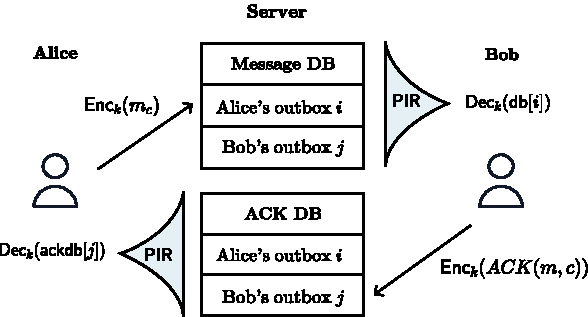
\includegraphics[width=0.7\textwidth]{ACK.pdf}
\caption{All server interactions for a message from Alice to Bob. }
\label{fig:pirandacks}
\end{figure}


Given the limited communication capacity, ACKs turn out to be slightly more subtle than this. In particular, if one user goes offline, we need to continue sending ACKs to them, which could potentially block other ACKs and slow down message transmission. Because each ACK only needs to encode two integers $(m, c)$, we can encode the ACKs for 20 contacts in one database row, which avoids this problem.
\section{Trust establishment}

Most existing metadata private messaging systems, such as Pung or Addra, assumes a prior key exchange between users. In our messaging system, we need a mechanism to conduct the key exchange itself while hiding the key exchange from everyone else. In other words, if Alice knows the public key $pk_B$ of Bob, then Alice should be able to send an ``invitation" to Bob. Bob must be able to retrieve this invitation from the server, and complete a key exchange with Alice. We call this process ``trust establishment".

This problem is known as Oblivious Message Detection(OMD) in \cite{liutromer2021}. The scheme proposed in \cite{liutromer2021} aims to minimize user download size, but it costs each user $\$ 1$ per million messages scanned, which is prohibitive for our messaging application. We provide two alternate methods of trust establishment with better computational cost and security.

In the following two methods, we assume that Alice and Bob's clients have generated a Curve25519 key exchange keypair $kx = (kx^P, kx^S)$.

\subsection{Face-to-face Invitations}
Our first method assumes that Alice and Bob are able to set up a face-to-face meeting with each other, either in person or over zoom. The trust establishment process is a simple key exchange implemented as follows.

1. Alice encodes her key exchange public key $kx_A^P$ and her allocation index $i_A$ into a human-readable story $s_A$. Bob similarly encodes his story $s_B$.

2. Alice and Bob meets and types the other's story into their own client. 

3. Alice decodes Bob's story to obtain $kx^P_B$ and $i_B$. She computes the shared secret $sk = DH(kx^P_B, kx^S_A)$, and adds $i_B$ to her set of listening indices.\todo{Better name?} Bob does the same. They can now communicate to each other using PIR.

Using this method, all interactions between the users do not require the internet. Thus, trust establishment can be completed instantly, cheaply, and securely. Our system do require Alice and Bob to be able to set up a meeting and type each other's story manually. To justify this approach, we believe a privacy-conscious Alice would be willing to set up a face-to-face meeting with Bob before sending him sensitive information.

\subsection{Asynchronous Invitation}

\todo{mention key privacy}

Our second method targets the case when Bob does not know about Alice's invitation beforehand. For example, Alice can be a sensitive client who wishes to privately reach out to Bob's company. 

This method proceeds in three steps: First, Alice sends an encrypted invitation to the server. Second, Bob retrieves this invitation via a full database download. Third, Bob informs Alice of his acceptance via an ACK message.

\textbf{To send an invitation}

1. Upon registration, each user's daemon generates an additional invitation keypair $ki = (ki^P, ki^S)$. Bob's daemon computes a ``public id" $id_B$, which contains his invitation public key $ki_B^P$, key exchange public key $kx_B^P$, and allocation $i_B$ encoded in plaintext. It then displays the id on Bob's GUI. Bob posts $id_B$ on his public profile, such as on twitter or on his company's website.

3. When Alice wishes to send an invitation to Bob, she obtains $id_B$ from Bob's public profile, and decodes it to obtain $(i_B, kx_B^P, ki_B^P)$. She drafts an initial message $m_{AB}$ to accompany her invitation. 

4. Alice's daemon periodically sends the key-value pair $(i_A, c_{AB} = \Enc(kx_B^P, id_A \vert m_{AB}))$ to the server\footnote{It is important to redo this encryption each round, otherwise adversaries will observe the same message repeatedly}, which stores it in a separate \textbf{AsyncInvitationDatabase}. When Alice has no invitations, her daemon sends $(i_A, \Enc(kx, id_A))$ for a random public key $kx$.

4. As Alice's daemon sends the invitation, it also compute the shared secret $sk = DH(kx_B^P, kx^S_A)$. It sends Bob a ``control message" $ctm_{AB}$ via the PIR database using $sk$, and adds $i_B$ to the set of listening indices.

\textbf{To retrieve an invitation}

1. Bob's daemon periodically downloads the entire \textbf{AsyncInvitationDatabase}. It computes $\Dec(kx^S_B, c)$ over all key-value pairs $(i, c)$. If the decryption fails, Bob's daemon ignores this pair. Now suppose $(i, c) = (i_A, c_{AB})$, and the decryption succeeds. Bob's daemon decodes $i = i_A, id_A, m_{AB}$ from the decrypted data, and displays on Bob's GUI that he received an incoming invitation from $id_A$ with message $m_{AB}$.

2. Bob verifies Alice's identity using $id_A$ and $m_{AB}$, for example by checking Alice's public profile. Bob then chooses to either accept or reject the invitation. If Bob rejects the invitation, no further action is performed. 

\textbf{To accept an invitation}

1. If Bob accepts Alice's invitation, Bob's daemon decodes $id_A$ to obtain $kx_A^P$, and computes the shared secret $sk = DH(kx_A^P, kx_B^S)$. It adds $i_A$ to the set of listening indices.

2. Since Alice is sending the control message $ctm_{AB}$ to Bob using the same shared secret $sk$, Bob's daemon will read $ctm_{AB}$ from the PIR database. It sends an ACK to Alice's control message.

3. When Alice's daemon reads Bob's ACK to $ctm_{AB}$ from the PIR ACK database, it displays on Alice's GUI that Bob has accepted Alice's friend request. Alice and Bob can now communicate to each other using PIR.

This method offers convenience on par with most existing messaging platforms. Its main disadvantage is cost and delay: downloading the entire database is expensive and time-consuming for user $B$. Furthermore, it makes user $B$ more difficult to ascertain that user $A$ is trustworthy, thus compromising $B$'s security. We discourage the use of this method, and allow users to disable it completely. \todo{Decision to figure out later?}
\todo{step-by-step guide?}
\todo{Not sure if this is going to be a thing for now.}
\section{Client-side security in practice}

The anysphere client is only as strong and secure as the most vulnerable part of our software supply chain. Software supply chains are an increasingly complex (and brittle) part of the software ecosystem because of a large and growing number of direct and transitive dependencies written across the world. 
The Anysphere client is designed to handle extreme private and critical communication securely, so our team has enforced a high bar of security for the core of our system. We focused on providing practical protection by significantly reducing the attack surface of our client, ensuring safe updates, and protecting against non-privileged software. 

A note on the client's security, in the context of our threat model: Anysphere trusts its client's devices. 
In particular, we trust that the local device is running a correct implementation of our protocol, and the computer comes without pre-installed backdoors. 
Our model is the bare minimum of trust we must assume, and we think this is reasonable given the intense focus of Apple and many other companies on device security. 
(Put another way, no encryption schemes we can come up with can secure our client inside a compromised computer.)
And with this context, we will present our measures to reduce the risk of a compromised Anysphere client.

\subsection{Reducing the Software Supply Chain attack surface}

We architected our client to consist of two parts: a UI frontend and a daemon backend, where the daemon backend contains all security-critical code. We sandbox the UI frontend in such a way that it is not allowed to talk to the internet, and let all message sending go through the daemon, which handles the cryptography. That way, even if there are bugs in the UI frontend, or potentially malicious code, there is not much it can do.

\todo{Figure of client architecture with UI and daemon, showing how we cut off internet access.}

We also reduce the attack surface of the daemon itself. In particular, we use C++ instead of other popular languages (Rust, Go, Python), because all other practical languages are significantly more susceptible to supply chain attacks. Our daemon has 4 direct dependencies (Abseil, gRPC, SQLite, Libsodium) and 0 transitive dependencies. A comparable implementation in a language with a package manager would easily use 100s of transitive dependencies. We elaborate more on our choice of C++ in this blog post \todo{Link.}.

% \subsection{Code distribution}

% We sign everything.

% Maybe we sign everything twice?

% Maybe we have a cold-storage and a hot-storage signing key?

% Do we store a backup key in cold storage that we can use to revoke a version? And people can disi

% \todo{Either understand whether standard OS signing is good enough, or whether we should sign things ourselves.}

\subsection{Updates}

Every update needs to be signed. In fact, it needs to be signed twice: Arvid holds one key, and Sualeh holds one key. Both signatures must be present for the local client to accept the update.

We implement our own signature check. Many popular frameworks have built-in signature checks, such as AutoUpdater for Electron and Updater for Tauri, but to ensure that we are really certain that updates work the way we want them to, we do it ourselves.

This means that if either of us loses our private key, you would not get any updates. This is by design.

\subsection{Protecting against non-privileged local malware}

If you've granted administrator access to a malicious program on your computer, there is, unfortunately, nothing to be done. We can, nevertheless, reduce the risk of non-privileged malware.

\todo{Actually implement: allow to encrypt the database, in which case the both the GUI and the CLI need to require passwords (and the GUI may cache the password for some amount of time).}

Again, we do not aim to eliminate the risk here. Non-privileged malware may still gather information from side-channel attacks, and potentially other avenues. Once an attacker has access to your computer, it is very, very hard to shield yourself from them.
\section{Related Research}

The research community has studied metadata-private communication for decades. In 1981, David Chaum introduced \textit{mix-nets}, which bounce messages between a small number of servers \cite{chaum1981untraceable}. Combined with onion encryption, mix-nets make it impossible to determine the destination of a given source packet, \textit{assuming that at least one server is honest}. Using mix-nets, Tor was created in 2002 and became one of the most successful privacy-protecting real-world projects \cite{dingledine2004tor}. Unfortunately, in addition to the server trust issue, mix-nets leak timing data, making it easy for someone with ISP-level network control to observe who is talking to whom. In today's world, it is getting easier and easier to amass enough data to perform such correlation attacks, making mix-net-based approaches unsuitable \cite{karunanayake2021anonymisation}.

Systems with stronger metadata-privacy guarantees saw a flurry of interest in the last decade: Dissent and Riposte  used so-called DC-nets \cite{corrigan2010dissent,corrigan2015riposte}, Vuvuzela, Atom, Talek and many others  introduced mix-nets with stronger security guarantees \cite{van2015vuvuzela,cheng2020talek,kwon2017atom}, Clarion, mcMix and Blinder introduced multi-party computation techniques \cite{alexopoulos2017mcmix,eskandarian2021clarion,abraham2020blinder}, and NIAR  introduced function-hiding functional encryption \cite{shi2021non,bunz2021non}.
All but NIAR's approach are less secure than our PIR-based approach, and NIAR is impractical at scale due to computation time.
The PIR line of work, started by Angel with Pung \cite{angel2016unobservable,angel2018pir} and continued by Addra \cite{ahmad2021addra}, promises both perfect security and reasonable scalability.

A communication system needs more than just message transmission. There has been much less attention in the literature to other components: establishing trust, managing many-to-many conversations, and defending against denial of service, to name a few. For trust establishment, Liu and Tromer recently initiated work on oblivious message retrieval \cite{liutromer2021}, which is unfortunately not scalable enough for us, but a good start to a field we want to develop further.
\section{What's Next?}\label{sec:future}

Private communication is a hard problem. We are actively doing research to increase convenience while preserving complete privacy. We also urge the research community to join us: during the first practical deployment of metadata-private communication, we have found that while many papers focus on the scalability of a core one-person messaging protocol, too few focus on problems that come up in practice, including private trust establishment, multiple-friend management, one-to-many and many-to-many communcation, and DoS protection.

% Anysphere has just begun operations, and we are devoted to truly free communication. 
% We aim to supervise and help build technologies that allow internet communication without unfair security assumptions.
% There are several important milestones that we have set for ourselves to reach to make this genuinely possible; some that are essential in the short-term and others that we want to achieve over a longer time horizon with time and effort.

\subsection{Implementation milestones}


\subsubsection{Small Files and images.} We hope to support the transmission of small files and images through our current protocol. 

\subsubsection{Forward secrecy.} We hope to integrate Signal's X3DH algorithm to ensure forward secrecy. 

\subsubsection{Public-key infrastructure.} To facilitate the discovery and .

\subsubsection{Calls.}

\subsubsection{Hardened daemon against local malware.}

\subsection{Research problems}

\subsubsection{Denial of service resistance.}

\subsubsection{One-to-many and many-to-many conversations.} An essentially important problem to solve is to allow groups of people to broadcast messages to each other, without depending on the presense of any specific user. We understand that this brings risks in itself to users because it increases the overall risk surface that a user has to trust but we believe it is crucial for large-scale pragmatic adoption.

\subsubsection{More efficient trust establishment.}

\subsubsection{The ACK problem.}

\subsubsection{The multiple friends problem.}

\subsubsection{Large Files and images.} Transmission of larger files and images is infeasible in our current framework because the number of chunks needed to deliver them is in the thousands; we will tackle that problem separately later.




\printbibliography


\end{document}
